\partsintesi{Síntesi de la Part I}{Aritmètica, Àlgebra i Trigonometria}


\begin{mylist}
	
\exer[2] Efectua les operacions següents i simplifica:
\begin{tasks}
	\task $\sqrt{a^3} - 2a \sqrt[4]{a^2} + 3a \sqrt[6]{a^3} - \sqrt[8]{a^{12}}$
	\task $\dfrac{5}{\sqrt{6}} + \dfrac{2}{\sqrt{6}+3\sqrt{2}} - \dfrac{4\sqrt{2}}{\sqrt{3}}$
\end{tasks}
\answers{a) $a\sqrt{a}$ \quad \quad b) $\frac{3\sqrt{2}-4\sqrt{6}}{6}$}

\exer[2] Efectua les operacions següents i simplifica:
\begin{tasks}(2)
	\task $\left( \sqrt[4]{a^3} \cdot \sqrt[5]{a^4} \right): \sqrt{a}$
	\task $\dfrac{4+\sqrt{6}}{2\sqrt{3}}  -  \dfrac{2}{3-\sqrt{3}}$
\end{tasks}
\answers{a) $a\,\sqrt[20]{a}$ \quad \quad b)$\frac{2\sqrt{3}+3\sqrt{2}-6}{6}$}

\exer[2] Factoritza el polinomi $3x^5 - 4x^4 - 5x^3 + 2x^2$
\answers{$x^2 (x+1) (x-2) (3x-1)$}

\exer[2] Opera i simplifica $\left( \dfrac{x^2-4}{x+1} : \dfrac{x^2+2x}{x^3-x} \right) - (x^2-3x)$
\answers{2}

\exer[2] Resol l'equació $\sqrt{2x+3} - 2x = x-6$
\answers{$x=3$ vàlida.}

\exer[2] Resol l'equació $\dfrac{7-x}{x^2+4x+4} + \dfrac{x}{x+2}=1$
\answers{$x=1$}

\exer[2] Resol el sistema d'inequacions $\left\{ \begin{array}{l} 
x+1-3(x-1)<1-x \\ x^2-x-6\ge 0 
\end{array}\right.$
\answers{$(3, +\infty)$}

%\exer[2] Resol pel mètode de Gauss $\left\{ \begin{array}{ll} 
%x+2y+z &=1 \\ -2x+y-z &= -5 \\ 3x-y+3z &=10 
%\end{array}\right.$
%\answers{$x=2$, $y=-1$, $z=2$}

\exer[2] Un examen consisteix en un test de 60 preguntes. Per cada encert obtens 5 punts, per cada errada et lleven 2 punts i per cada pregunta no contestada resta 1 punt. Quantes preguntes bé, malament i en blanc va contestar un alumne sabent que va obtenir 150 punts i que el nombre d'errades més el quíntuple de les no contestades va ésser igual al nombre d'encerts? 
\answers{$x=38$: be, $y=18$: malament, $z=4$: no contestades. Planteig: $x+y+z=60$; $5x-2y-z=150$; $y+5z=x$}

\exer[2] Resol pel mètode de Gauss i classifica el sistema $\left\{ \begin{array}{ll} 
2x+y-z &=-1 \\ x-y+z &= 4 \\ 4x-y+z &=7 
\end{array}\right.$
\answers{S.C.I. $x=1$, $y=z-3$, $z=z$}

\exer[2] Les diagonals d'un paral·lelogram mesuren 16 cm i 28 cm i formen un angle de 48º. Calcula el perímetre i l'àrea d'aquest paral·lelogram.
\answers{Els costats són 10.49 cm i 20.25 cm, el perímetre 61.48 cm. L'àrea 83.23 cm$^2$.}
 
\exer[2] Tenim un triangle de perímetre 48 cm. Sabent que el costat major supera en 6 unitats el menor i que l'altre costat és la mitjana aritmètica del major i del menor, calcula els angles d'aquest triangle.
\answers{Primer obtenim els costats resolent un sistema d'equacions $a=19$,  $b=16$ i $c=13$. Després aplicam el Teorema del Cosinus per obtenir els angles $\hat A=42.54^\circ$, $\hat B=56.3^\circ$, $\hat C=81.17^\circ$}

\exer[2] 
\begin{minipage}[t]{0.55\textwidth}
Per construir un túnel entre dues ciutats $A$ i $C$ necessitam saber la seva longitud i direcció. Per això, fixam un punt $B$ i prenem les mesures indicades en la figura. Calcula $\bar{AC}$ i els angles $\hat B$ i $\hat C$.
\end{minipage}
\begin{minipage}[c]{0.5\textwidth}
\begin{center}
	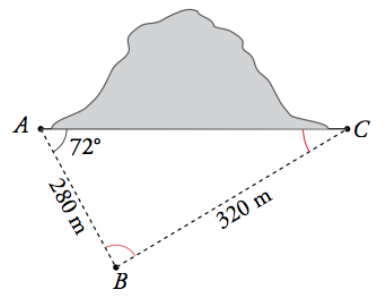
\includegraphics[width=5cm]{img-04-bloc1/bloc1-fig1.png}
\end{center}
\end{minipage}
\answers{Utilitzam el Teorema del Sinus. $\hat C= 56^\circ \, 19^\prime \, 31^{\prime\prime}$, $\hat B= 51^\circ \, 40^\prime \, 29^{\prime\prime}$ i  $\bar{AC}=263.96$ m.}

\exer[2] Una nau espacial es troba sobrevolant el pol nord de la Terra a una certa distància $d$ de la seva superfície. Si volem veure els continents fins a una latitud de $40^\circ$ nord, quina és l'altura mínima ha de volar la nau? Preneu radi de la Terra $R=6400$ km.
\answers{$d=3557$ km sobre la superfície de la Terra.} 

\exer[2] Justifica si existeix algun angle $a$ pel qual $\tg a=\frac{2}{3}$ i $\sin a = \frac{1}{2}$.
\answers{No existeix cap angle amb aquestes condicions. S'obtindria que $\cos a = 3/4$ i amb aquesta dada no es compleix que $\sin^2 a +\cos^2 a = 1$.}

\exer[2] Sabent que $\tg \alpha= 2$ i que $\cos \alpha>0$, troba:
\begin{tasks}(4)
	\task $\cos 2\alpha$
	\task $\sin(\frac{\pi}{2}-\alpha)$
	\task $\sin \frac{\alpha}{2}$
	\task $\tg (\frac{\pi}{4}+\alpha)$
\end{tasks}
\answers{En primer lloc trobam que $\sin \alpha = \frac{2\sqrt 5}{5}$ i $\cos \alpha = \frac{\sqrt 5}{5}$. 	a) $-3/5$ \quad   b) $\frac{\sqrt 5}{5}$ \quad  c)  $\sqrt{\frac{5-\sqrt 5}{10}}$ \quad  d) $-3$}

\exer[2] Demostra les següents identitats trigonomètriques
\begin{tasks}
	\task $\cos^4 \alpha - \sin^4 \alpha = 2 \cos^2 \alpha -1$
	\task $2 \tg \beta \cdot \cos^2 \frac{\beta}{2}-\sin\beta = \tg \beta$
\end{tasks}
\answers{a) Utilitza que $sin^4 x = (1-\cos^2 x)^2$ desenvolupa el quadrat i simplifica.
	b) Utilitza que $\cos^2 \frac{\beta}{2} = \frac{1+\cos \beta}{2}$
}

\exer[2] Resol aquestes equacions trigonomètriques
\begin{tasks}
	\task $2\sin x + \cos x = 1$
	\task $2 \sin^2 \frac{x}{2} + \cos 2x = 0$
\end{tasks}
\answers{a) $x= 0^\circ+ n\cdot 360^\circ$, $x=126.87^\circ+ n\cdot 360^\circ$. 
	b) $x= 90^\circ+ n\cdot 180^\circ$, $x= 60^\circ+ n\cdot 360^\circ$, $x= 300^\circ+ n\cdot 360^\circ$.}

\exer[2] Resol $\left\{ \begin{array}{l}  
\sin 3x + \sin y = \frac{3}{2} \\ 
\cos \left(  \frac{3x-y}{2} \right) = \frac{\sqrt{3}}{2}
\end{array}\right.$
\answers{$x=30^\circ + n\cdot 180^\circ$, $y=30^\circ + k\cdot 180^\circ$.}

\exer[2] Efectua $\dfrac{(3-2i)^2 - (1+i)(2-i)}{-3+i}$
\answers{$-\frac{19}{10}+\frac{37}{10}i$}

\exer[2] Simplifica $\dfrac{i^{10} - 2 i^7}{2 + i^{33}}$. \emph{Ajuda: Recorda quines són les potències de} $i$.
\answers{$i$}

\exer[2] Resol l'equació en el conjunt dels nombres complexos $z^2-10z+29=0$.
\answers{$z=5+2i$, $z=5-2i$}

\exer[2] Donat el nombre complex $z=3_{\, 60^\circ}$, expressa en forma polar $z^*$, $1/z$, $z^2$, $\sqrt[3]{z}$. 
\answers{ $z^*=3_{\, 300^\circ}$, $1/z=(1/3)_{\, 300^\circ}$, $z^2=9_{\, 120^\circ}$, $\sqrt[3]{z}$ té tres resultats = $(\sqrt{3})_{\, 20^\circ}$, $(\sqrt{3})_{\, 140^\circ}$ i $(\sqrt{3})_{\, 260^\circ}$.}
\end{mylist}
